\documentclass[10pt]{article}
\usepackage[margin=12mm]{geometry}
\usepackage{graphicx}
\usepackage{caption}
\usepackage{tikz}
\pagestyle{empty}
\captionsetup{font=small,labelfont=bf}

\begin{document}
\begin{figure}[p]
\centering
\resizebox{\textwidth}{!}{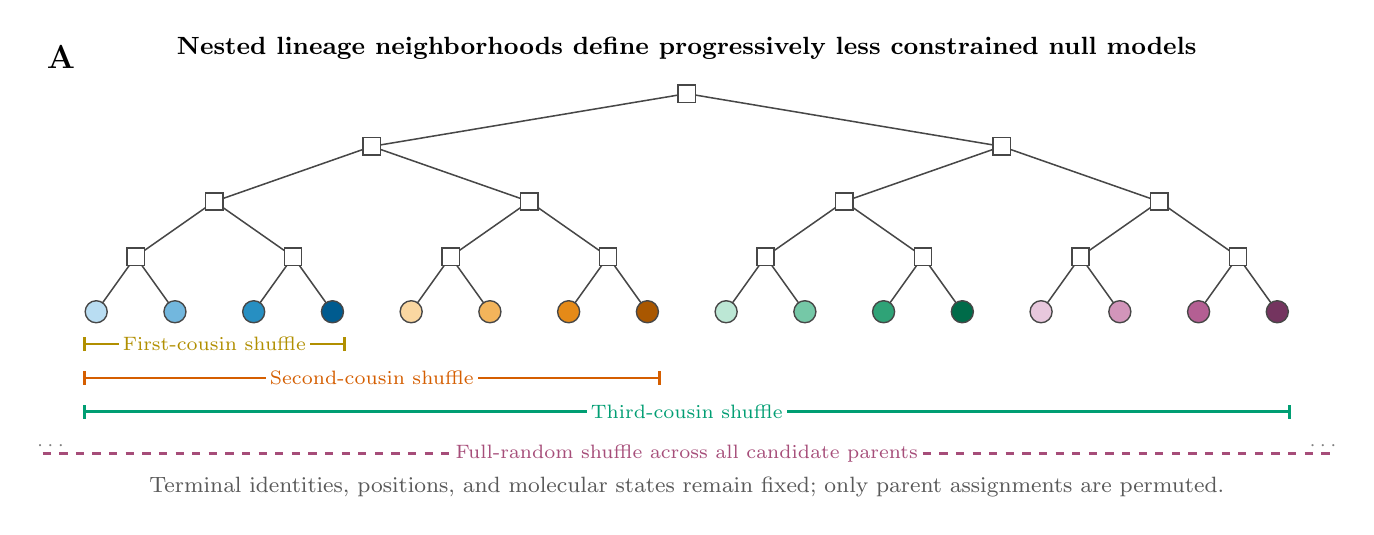
\begin{tikzpicture}[
  x=1cm,y=1cm,
  lineage/.style={draw=black!72,line width=0.55pt},
  nodebox/.style={rectangle,draw=black!72,fill=white,
                  minimum size=2.2mm,inner sep=0pt,line width=0.5pt},
  terminal/.style={circle,draw=black!72,minimum size=2.8mm,
                   inner sep=0pt,line width=0.5pt},
  every node/.style={font=\sffamily},
]
\definecolor{blueOne}{HTML}{B9DDF2}
\definecolor{blueTwo}{HTML}{72B7DE}
\definecolor{blueThree}{HTML}{278FC2}
\definecolor{blueFour}{HTML}{005B8F}
\definecolor{orangeOne}{HTML}{FAD7A1}
\definecolor{orangeTwo}{HTML}{F3B45B}
\definecolor{orangeThree}{HTML}{E58A18}
\definecolor{orangeFour}{HTML}{A95700}
\definecolor{greenOne}{HTML}{BCE7D5}
\definecolor{greenTwo}{HTML}{75C8A7}
\definecolor{greenThree}{HTML}{2FA377}
\definecolor{greenFour}{HTML}{006B49}
\definecolor{purpleOne}{HTML}{E8C8DD}
\definecolor{purpleTwo}{HTML}{D295BA}
\definecolor{purpleThree}{HTML}{B45F93}
\definecolor{purpleFour}{HTML}{74345F}
\definecolor{firstCol}{HTML}{B18F00}
\definecolor{secondCol}{HTML}{D55E00}
\definecolor{thirdCol}{HTML}{009E73}
\definecolor{fullCol}{HTML}{A64D79}

\node[font=\bfseries\large,anchor=north west] at (-0.25,5.25) {A};
\node[font=\bfseries\small] at (8.0,5.10)
  {Nested lineage neighborhoods define progressively less constrained null models};

% A balanced four-level example lineage with 16 terminal identities.
\foreach \x/\name in {0.5/t1,1.5/t2,2.5/t3,3.5/t4,4.5/t5,5.5/t6,
  6.5/t7,7.5/t8,8.5/t9,9.5/t10,10.5/t11,11.5/t12,
  12.5/t13,13.5/t14,14.5/t15,15.5/t16}
  \coordinate (\name) at (\x,1.75);
\foreach \x/\name in {1/p1,3/p2,5/p3,7/p4,9/p5,11/p6,13/p7,15/p8}
  \coordinate (\name) at (\x,2.45);
\foreach \x/\name in {2/g1,6/g2,10/g3,14/g4}
  \coordinate (\name) at (\x,3.15);
\coordinate (a1) at (4,3.85);
\coordinate (a2) at (12,3.85);
\coordinate (root) at (8,4.52);

\draw[lineage] (root)--(a1) (root)--(a2)
  (a1)--(g1) (a1)--(g2) (a2)--(g3) (a2)--(g4)
  (g1)--(p1) (g1)--(p2) (g2)--(p3) (g2)--(p4)
  (g3)--(p5) (g3)--(p6) (g4)--(p7) (g4)--(p8)
  (p1)--(t1) (p1)--(t2) (p2)--(t3) (p2)--(t4)
  (p3)--(t5) (p3)--(t6) (p4)--(t7) (p4)--(t8)
  (p5)--(t9) (p5)--(t10) (p6)--(t11) (p6)--(t12)
  (p7)--(t13) (p7)--(t14) (p8)--(t15) (p8)--(t16);
\foreach \n in {root,a1,a2,g1,g2,g3,g4,p1,p2,p3,p4,p5,p6,p7,p8}
  \node[nodebox] at (\n) {};

\foreach \n/\c in {t1/blueOne,t2/blueTwo,t3/blueThree,t4/blueFour,
  t5/orangeOne,t6/orangeTwo,t7/orangeThree,t8/orangeFour,
  t9/greenOne,t10/greenTwo,t11/greenThree,t12/greenFour,
  t13/purpleOne,t14/purpleTwo,t15/purpleThree,t16/purpleFour}
  \node[terminal,fill=\c] at (\n) {};

% Nested shuffle domains, following the visual language of the talk schematic.
\draw[firstCol,line width=1.0pt] (0.35,1.25)--(0.35,1.43)
  (0.35,1.34)--(3.65,1.34) (3.65,1.25)--(3.65,1.43);
\node[font=\scriptsize,text=firstCol,fill=white,inner sep=1.5pt]
  at (2.0,1.34) {First-cousin shuffle};

\draw[secondCol,line width=1.0pt] (0.35,0.82)--(0.35,1.00)
  (0.35,0.91)--(7.65,0.91) (7.65,0.82)--(7.65,1.00);
\node[font=\scriptsize,text=secondCol,fill=white,inner sep=1.5pt]
  at (4.0,0.91) {Second-cousin shuffle};

\draw[thirdCol,line width=1.0pt] (0.35,0.39)--(0.35,0.57)
  (0.35,0.48)--(15.65,0.48) (15.65,0.39)--(15.65,0.57);
\node[font=\scriptsize,text=thirdCol,fill=white,inner sep=1.5pt]
  at (8.0,0.48) {Third-cousin shuffle};

\node[font=\scriptsize,text=black!50] at (-0.08,0.04) {$\cdots$};
\node[font=\scriptsize,text=black!50] at (16.08,0.04) {$\cdots$};
\draw[fullCol,line width=1.0pt,dashed] (-0.18,-0.05)--(16.18,-0.05);
\node[font=\scriptsize,text=fullCol,fill=white,inner sep=1.5pt]
  at (8.0,-0.05) {Full-random shuffle across all candidate parents};

\node[font=\footnotesize,text=black!65] at (8.0,-0.48)
  {Terminal identities, positions, and molecular states remain fixed; only parent assignments are permuted.};
\end{tikzpicture}
}

\vspace{4mm}
\begin{minipage}[t]{0.485\textwidth}
  \centering
  \includegraphics[width=\linewidth]{terminal_support_B_er_td.pdf}
\end{minipage}\hfill
\begin{minipage}[t]{0.485\textwidth}
  \centering
  \includegraphics[width=\linewidth]{terminal_support_C_structural_retention.pdf}
\end{minipage}

\caption{\textbf{Null models and structural metrics along the terminal-cell Pareto front.}
\textbf{A,} Nested cousin-shuffling null models progressively relax the
lineage restriction on terminal cell to parent assignments. First-cousin
shuffling acts within the smallest neighborhoods, second- and third-cousin
shuffling act within successively larger ancestral neighborhoods, and full-random
shuffling permits assignments among all candidate parents. Terminal-cell
identities, i.e., their final positions, and molecular states remain fixed.
\textbf{B,} Edge retention (blue, left axis) and mean lineage-tree distance
among changed edges (grey, inverted right axis) compared with the natural
lineage for all assignments along the Pareto front. The natural lineage has
edge retention one and, by definition, no changed edges; it is shown at the
zero-distance reference. Markers identify the natural lineage, the
maximum-edge-retention assignment, and the minimum-tree-distance assignment.
Marks on the right axis show the corresponding changed-edge mean tree distances
under first-cousin and full-random shuffling.
Approaching either single-objective optimum requires increasingly significant
changes from the natural lineage.
\textbf{C,} Structural retention while moving along the Pareto front from
the maximum-edge-retention compromise toward either single-objective
optimum. The inset indicates the direction of travel of the two colored
trajectories along the Pareto front. For each trajectory separately, the
horizontal axis reports the fraction of the attainable reduction in its
corresponding distance; this normalization does not compare or combine the
objectives. Natural-edge retention falls as the remaining benefit is pursued.
The shaded final 5\% of attainable distance reduction costs a further 5.4 percentage
points of edge retention and 0.7 mean tree-distance units toward the travel optimum,
and 11.4 percentage points and 2.0 tree-distance units toward the cell-state optimum.}
\label{fig:ce-terminal-pareto-supporting}
\end{figure}
\end{document}
